% Template for Cogsci submission with R Markdown

% Stuff changed from original Markdown PLOS Template
\documentclass[10pt, letterpaper]{article}

\usepackage{cogsci}
\usepackage{pslatex}
\usepackage{float}
\usepackage{caption}

% amsmath package, useful for mathematical formulas
\usepackage{amsmath}

% amssymb package, useful for mathematical symbols
\usepackage{amssymb}

% hyperref package, useful for hyperlinks
\usepackage{hyperref}

% graphicx package, useful for including eps and pdf graphics
% include graphics with the command \includegraphics
\usepackage{graphicx}

% Sweave(-like)
\usepackage{fancyvrb}
\DefineVerbatimEnvironment{Sinput}{Verbatim}{fontshape=sl}
\DefineVerbatimEnvironment{Soutput}{Verbatim}{}
\DefineVerbatimEnvironment{Scode}{Verbatim}{fontshape=sl}
\newenvironment{Schunk}{}{}
\DefineVerbatimEnvironment{Code}{Verbatim}{}
\DefineVerbatimEnvironment{CodeInput}{Verbatim}{fontshape=sl}
\DefineVerbatimEnvironment{CodeOutput}{Verbatim}{}
\newenvironment{CodeChunk}{}{}

% cite package, to clean up citations in the main text. Do not remove.
\usepackage{apacite}

% KM added 1/4/18 to allow control of blind submission


\usepackage{color}

% Use doublespacing - comment out for single spacing
%\usepackage{setspace}
%\doublespacing


% % Text layout
% \topmargin 0.0cm
% \oddsidemargin 0.5cm
% \evensidemargin 0.5cm
% \textwidth 16cm
% \textheight 21cm

\title{Combinatorial Capacity of English Negation in Child Language}


\author{{\large \bf Morton Ann Gernsbacher (MAG@Macc.Wisc.Edu)} \\ Department of Psychology, 1202 W. Johnson Street \\ Madison, WI 53706 USA \AND {\large \bf Masoud Jasbi (jasbi@ucdavis.edu)} \\ Department of Linguistics, 469 Kerr Hall, One Shields Avenue \\ Davis, CA 95 USA}


\begin{document}

\maketitle

\begin{abstract}
Negation is very important for langauge and thought. How does it develop
in the language of children? There has been many guessses like
rejection, non-existence, denail, etc. but it has been hard to assess
because these concepts are vaguge. Here we assess the combinatorial
capacity of early negation in children's productions, and use words
negation combines with as a proxy for early concepts expressed by it. We
show some important stuff.

\textbf{Keywords:}
Add your choice of indexing terms or keywords; kindly use a semi-colon;
between each term.
\end{abstract}

\hypertarget{introduction}{%
\section{Introduction}\label{introduction}}

Negation is an abstract concept, lexicalized in all previously studied
human languages, and crucial to everyday communication. It can help a
coffee shop divide its menu into ``coffee'' and ``not coffee'' sections,
with the ``not coffee'' section bringing together diverse items that
otherwise cannot be labeled. It can help us regulate others' actions in
a sign like ``no mask, no entry''. It can also communicate our deepest
wants and dislikes. But how does this crucial abstract concept emerge in
humans? Does language play a role in its emergence or does language
simply adopt it for communication?

There has been several influential hypotheses on the conceptual origin
of negation.

In this paper, we address the same issues with a slightly different
approach. We start with the widely accepted assumption that negation is
a higher order operator or function, operating on lower level concepts.
The question we ask is: what type of concepts does linguistic negation
operate on in early child language? Do we find negation starting in a
limited conceptual domain and then expanding to others? Or do we find it
operating across different conceptual domains as early as we can attest
it?

Darwin (1998) thought that negation has roots in the expression of human
emotions and desires. He hypothesized that the earliest manifestation of
negation and affirmation in infants is when they refuse food from
parents, by withdrawing their heads laterally, or when they accept the
food, by inclining their heads forward. He suggested that head shaking
and nodding as common gestures for negation and affirmation have
developed from this early habit. Considering early functions of negative
morphemes like \emph{no}, many researchers proposed that children use
them to ``reject'' or ``refuse'' (Bloom, 1970; Choi, 1988; Pea, 1978).
For example, they may say ``no'' when asked ``do you want juice?'', say
``not want it'', or say ``don't like it''. Pea (1978) proposed that this
function of negation is the first to emerge in children.

Motor control: prohibition (do not spill milk), inability (I cannot zip
it)

Bloom (1970) suggested that the first function of negation in children's
speech is to express non-existence. Relates to children's development of
object permanence.

Perceptual: non-existence (no juice, no more milk, no fish in the
bathroom, I do not have underpants), failure, Locatives (no in there,
daddy was not on the phone), non-events (the dog not barking)

A third possible domain and path to the acquisition of negation is
language itself. Word learning places its own constraints on the
conceptual space. One possibility is that negation develops, and is
aided by the act of labeling and categorizing objects and actions for
linguistic communication. This function would manifest istelf in
labeling acts with nominal predicates such as ``this is not a bunny'',
``not red'', or ``this isn't a reptile''.

There has been no proposal for negation originating in the child's
understanding of her own or other's epistemic states. In fact, most
development theory of mind accounts assume that this ability emerges
later in children. However, many corpus instances of negation modify
mental state verbs such as \emph{know}, \emph{think}, and
\emph{remember} (e.g.~``I not know''). Therefore, we also report the
prevalence and emergence of such cases.

Caveat on production vs comprehension.

\hypertarget{experiments}{%
\section{Experiments}\label{experiments}}

\hypertarget{data-and-preprocessing}{%
\subsection{Data and preprocessing}\label{data-and-preprocessing}}

For developmental data of child language in English, we turned to the
CHILDES database (MacWhinney, 2000), which provides child-parent
conversational interactions. We focused on utterances produced by
children with typical development within the age range of 12 - 72
months, then extracted cases with any of the three negation markers that
are of interest in this study: \emph{no}, \emph{not} and \emph{n't}.
Utterances with only one lexical token (e.g.~\emph{no !}) were not
considered as here we aim to address particularly the question of what
negation markers could \emph{combine} with. Preprocessing led to a data
set of 365,260 utterances with negation structures from a total of 811
children across 56 corpora.

Figure @ref(fig:speaker\_stats)

\begin{CodeChunk}
\begin{figure}[H]

{\centering 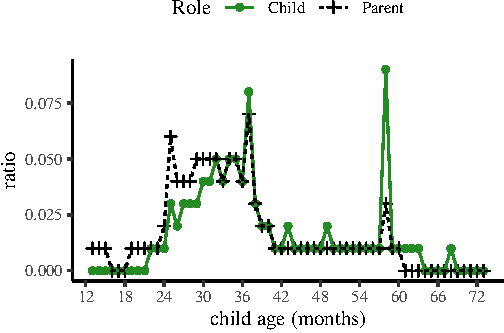
\includegraphics{figs/speaker_stats-1} 

}

\caption[Distribution of the number of utterances with negative morphemes in child and parent speech]{Distribution of the number of utterances with negative morphemes in child and parent speech.}\label{fig:speaker_stats}
\end{figure}
\end{CodeChunk}

\hypertarget{negation-concepts}{%
\subsection{Negation concepts}\label{negation-concepts}}

In this section, we describe in details our automatic extraction of
syntactic structures that express different types of negation concepts.
The current English data from CHILDES contains morphosyntactic
information (Sagae, Davis, Lavie, MacWhinney, \& Wintner, 2010) such as
part-of-speech (POS) information as well as grammatical or syntactic
dependency relations. We take advantage of information as such when
automatically identifying our constructions of interest. An utterance
with negative morpheme(s) was only considered when the negative
morphemes has either a POS of \emph{neg} or \emph{qn}, the latter of
which was mainly for cases with \emph{no} as a quantifier. Furthermore,
the syntactic functions and relations of the negative morphemes should
not be enumeration (\emph{no no no}), communicators or discourse markers

After extracting all instances with negative morphemes, the
developmental trajectory of each construction type as described in the
previous section was analyzed. While the matter of interest here is
child speech, we also compared patterns in child production to those in
parent speech as references at the corresponding age of the child. Then
we combined the development of all construction types for analysis as a
whole

\hypertarget{emotion}{%
\subsubsection{Emotion}\label{emotion}}

In order to investigate utterances that express emotions, particularly
the concept of rejections, we focused on specific cases where the head
verb of the phrase is either \emph{like} or \emph{want} (including
different forms of the verbs such as \emph{liked} or \emph{wanna} ), and
the head verb is immediately preceded by one of the three negative
morphemes. In particular, to not confuse with cases such as rhetorical
questions (\emph{don't you like it}) or declaratives (\emph{you don't
wanna do that}), which are more common in parent speech, our analyses
were restricted to utterances where the head verb \emph{like} or
\emph{want} takes either a subject \emph{I} or has no subject. The
existence of a subject was determined via searching for a word in the
utterance that has the \emph{SUBJ} dependency relation with the head
verb. Overall our data extraction resulted in a total of 12,329
utterances (Child: 8,223; Parent: 4,106). ~ (1) \emph{like}: \emph{I no
like sea} (2) \emph{want}: \emph{no want one now} / \emph{don't wanna
go} ~

To compare the patterns between child and parent speech, for each
domain, we calculated the relative ratio of (i) each of the three
negative morphemes overall; (ii) usage of negative morphemes with the
two different head verbs; (iii) utterances expression emotion with the
three negative morphemes at different ages of the child. In both child
and parent speech, when expressing emotion with either of the two head
verbs \emph{like} and \emph{want}, the most frequently used negative
morpheme is \emph{n't} combined with an auxiliary verb. Comparing the
two different head verbs, overall the negative morphemes are co-occur
with \emph{want} more frequently.

On the other hand, when looking at the developmental trajectory, as
presented in Figure @ref\{fig:emotion\}, children's usage of negative
morphemes is comparable regardless of the particular head verb. In
general, children did not start using negative morphemes in this domain
until the age of 7 months; their usage of these morphemes for the
concept of rejection is the most frequent during the age range of 13 -
21 months, then gradualy decreases as they age.

\begin{CodeChunk}
\begin{figure}[H]

{\centering 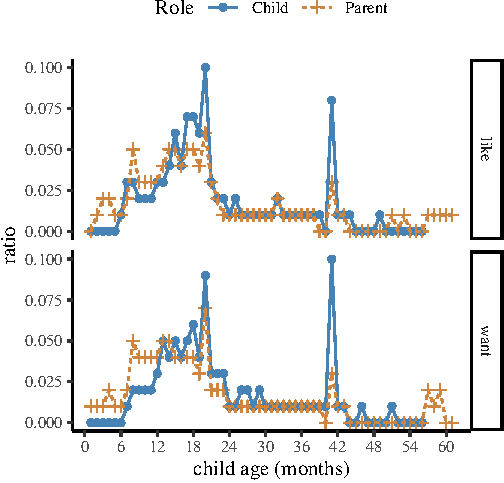
\includegraphics{figs/emotion-1} 

}

\caption[Emotion]{Emotion}\label{fig:emotion}
\end{figure}
\end{CodeChunk}

\hypertarget{motor-control}{%
\subsubsection{Motor control}\label{motor-control}}

For utterances that articulate the concept of motor control, we focused
on two individual aspects with different communicative functions. The
first one includes cases that indicate prohibition (\emph{e.g.} (3)),
and the second one contain cases that articulate inability (\emph{e.g.}
(4)). For the former, we analyzed cases where the negative morphemes are
combined with the auxiliary verb \emph{do} (\emph{do}, \emph{does},
\emph{did}) and the auxiliary does not take any subject; whereas for the
latter, we analyzed cases where the negative morphemes co-occur with the
auxiliary \emph{can} (\emph{can} and \emph{could}). For inability in
particular, similarly to the extraction of utterances that express
rejection, in order to not accidentally include utterances such as
rhetorical questions or imperatives (\emph{you can't do that}), we
excluded instances where the subject is not \emph{I}. This led to a
subset of 64,801 utterances (Child: 20,129; Parent: 44,672). ~ (3)
\emph{do}: \emph{don't blame Charlotte} (4) \emph{can}: \emph{I can't
see} ~

Again for comparison of child and parent speech, we calculated the
relative ratio of (i) each of the three negative morphemes overall; (ii)
usage of negative morphemes with the two different communicative
functions; (iii) utterances expression motor control with the three
negative morphemes at different ages of the child. Overall the most
frequently used negative morpheme is \emph{n't} when applied in the
domain of motor control. Comparing the two communicative functions, the
negative morphemes tend to co-occur more often when expressing
inability.

As shown in Figure @ref\{fig:motor\_control\}, the developmental
trajectory of using the negative morphemes in the domain of motor
control is similar to that in the domain of emotion. Children started
combining negative morphemes in syntactic structures that epxress
prohibiiton and inability around the age of 6 months, then gradually
increases until the age of 22 months.

\begin{CodeChunk}
\begin{figure}[H]

{\centering 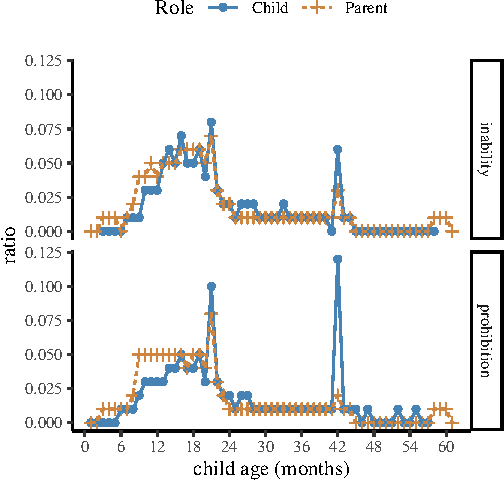
\includegraphics{figs/motor_control-1} 

}

\caption[Motor control]{Motor control}\label{fig:motor_control}
\end{figure}
\end{CodeChunk}

\hypertarget{language-learning}{%
\subsubsection{Language learning}\label{language-learning}}

Within the domain of language learning, we concentrated on cases where
negative morphemes are adopted to for labeing in the identity
(\emph{e.g.} (5) \& (6)) or existence (\emph{e.g.} (7)) of the nominal
object that is being described. To do this, we extracted utterances that
fit the following criteria: first, the negative morpheme has to be
modifying a copula verb; secondly, the copula verb has to have a
predicative nominal, which was identified with the help of POS
information and dependency relation. The POS of the predicate has to be
noun (\emph{n}) and its dependency relation with the copula has to be
\emph{PRED}. This resulted in a total of 12,739 utterances (Child: 3,350
utterances; Parent: 9,389 utterances). ~ (5) \emph{that's not a farmer}
(6) \emph{I'm not a heavy baby Mum} (7) \emph{can}: \emph{there are no
trees} ~

Again for comparison of child and parent speech, we calculated the
relative ratio of (i) each of the three negative morphemes overall; (ii)
usage of negative morphemes with the two different communicative
functions; (iii) utterances expression motor control with the three
negative morphemes at different ages of the child. Overall the most
frequently used negative morpheme is \emph{n't} when applied in the
domain of motor control. Comparing the two communicative functions, the
negative morphemes tend to co-occur more often when expressing
inability.

Comparing the three negative morphemes, the most frequently used is
\emph{not} in both child and parent speech. Based on results from Figure
@ref\{fig:learning\}, the developmental trajectory of using the negative
morphemes in the domain of language learning is comparable to previous
domains. Children started using the negative morphemes for the function
of labeling nominal objects around the age of 7 months and their usage
as such became more regular around the age of 10 months. However, the
frequency of applying the negative morphemes in the language learning
domain began to decrease around the age of 18 months.

\begin{CodeChunk}
\begin{figure}[H]

{\centering 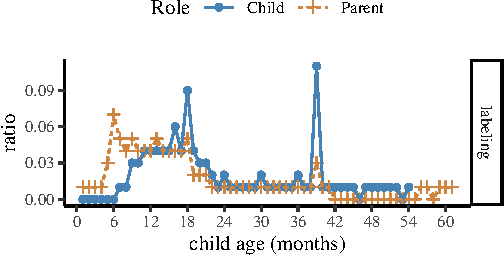
\includegraphics{figs/learning-1} 

}

\caption[Language learning]{Language learning}\label{fig:learning}
\end{figure}
\end{CodeChunk}

\hypertarget{theory-of-mind}{%
\subsubsection{Theory of mind}\label{theory-of-mind}}

With regards to the domain of theory of mind, we attended to cases that
express epistemic position. Specifically, we focused on utterances that
articulate the concept of unknowing (\emph{I not know} or \emph{I didn't
remember}) or uncertainty (\emph{I don't think so}). The cases that were
subject to analyses here included either \emph{know}, \emph{remember} or
\emph{think} as the head verb, modified by the negative morphemes or the
combination of the negative morphemes with auxiliaries. Additionally, we
restricted to instances where the head verb is either subjectless or has
the subject \emph{I}. This led to a subset of 27,821 utterances in total
(Child: 9,282; Parent: 18,539)

In both child and parent speech, the most frequently used negative
morpheme in expressing epistemic position is \emph{n't}, a pattern that
is consistent across the three different head verbs. And the negative
morphemes tend to co-occur more often in cases that describes the state
of unknowing, which is indicated mainly by the verb \emph{know}. Given
results from Figure @ref\{fig:epistemic\}, there does not seem to be a
quite consistent developmental trajectory of child speech in the domain
of theory of mind. While regardless of the head verb, children appeared
to start applying the negative morphemes in this domain around the age
of 4. Nevertheless, there seems to be more variability in expressing an
epistemic position with \emph{remember} and \emph{think} as the children
age. By contrast, the pattern for instances with \emph{know} gradually
decreases after the age of 16 months.

\begin{CodeChunk}
\begin{figure}[H]

{\centering 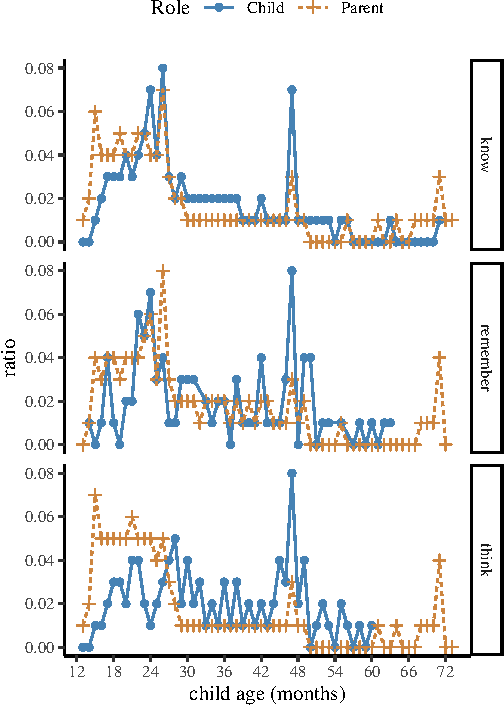
\includegraphics{figs/epistemic-1} 

}

\caption[Theory of mind]{Theory of mind}\label{fig:epistemic}
\end{figure}
\end{CodeChunk}

\hypertarget{an-overall-look-at-all-domains}{%
\subsubsection{An overall look at all
domains}\label{an-overall-look-at-all-domains}}

\hypertarget{study}{%
\section{Study}\label{study}}

First level headings should be in 12 point , initial caps, bold and
centered. Leave one line space above the heading and
1/4\textasciitilde line space below the heading.

\hypertarget{method}{%
\subsection{Method}\label{method}}

Second level headings should be 11 point , initial caps, bold, and flush
left. Leave one line space above the heading and 1/4\textasciitilde{}
line space below the heading.

\hypertarget{third-level-headings}{%
\subsubsection{Third-Level Headings}\label{third-level-headings}}

Third-level headings should be 10 point , initial caps, bold, and flush
left. Leave one line space above the heading, but no space after the
heading.

\hypertarget{discussion}{%
\section{Discussion}\label{discussion}}

Use standard APA citation format. Citations within the text should
include the author's last name and year. If the authors' names are
included in the sentence, place only the year in parentheses, as in
(1972), but otherwise place the entire reference in parentheses with the
authors and year separated by a comma (Newell \& Simon, 1972). List
multiple references alphabetically and separate them by semicolons
(Chalnick \& Billman, 1988; Newell \& Simon, 1972). Use the et.
al.~construction only after listing all the authors to a publication in
an earlier reference and for citations with four or more authors.

For more information on citations in RMarkdown, see
\textbf{\href{http://rmarkdown.rstudio.com/authoring_bibliographies_and_citations.html\#citations}{here}.}

\hypertarget{footnotes}{%
\subsection{Footnotes}\label{footnotes}}

Indicate footnotes with a number\footnote{Sample of the first
footnote.} in the text. Place the footnotes in 9 point type at the
bottom of the page on which they appear. Precede the footnote with a
horizontal rule.\footnote{Sample of the second footnote.} You can also
use markdown formatting to include footnotes using this
syntax.\footnote{Sample of a markdown footnote.}

\hypertarget{figures}{%
\subsection{Figures}\label{figures}}

All artwork must be very dark for purposes of reproduction and should
not be hand drawn. Number figures sequentially, placing the figure
number and caption, in 10 point, after the figure with one line space
above the caption and one line space below it. If necessary, leave extra
white space at the bottom of the page to avoid splitting the figure and
figure caption. You may float figures to the top or bottom of a column,
or set wide figures across both columns.

\hypertarget{two-column-images}{%
\subsection{Two-column images}\label{two-column-images}}

You can read local images using png package for example and plot it like
a regular plot using grid.raster from the grid package. With this method
you have full control of the size of your image. \textbf{Note: Image
must be in .png file format for the readPNG function to work.}

You might want to display a wide figure across both columns. To do this,
you change the \texttt{fig.env} chunk option to \texttt{figure*}. To
align the image in the center of the page, set \texttt{fig.align} option
to \texttt{center}. To format the width of your caption text, you set
the \texttt{num.cols.cap} option to \texttt{2}.

\begin{CodeChunk}
\begin{figure*}[h]

{\centering 
\includegraphics{figs/2-col-image-1} 

}

\caption[This image spans both columns]{This image spans both columns. And the caption text is limited to 0.8 of the width of the document.}\label{fig:2-col-image}
\end{figure*}
\end{CodeChunk}

\hypertarget{one-column-images}{%
\subsection{One-column images}\label{one-column-images}}

Single column is the default option, but if you want set it explicitly,
set \texttt{fig.env} to \texttt{figure}. Notice that the
\texttt{num.cols} option for the caption width is set to \texttt{1}.

\begin{CodeChunk}
\begin{figure}[H]

{\centering 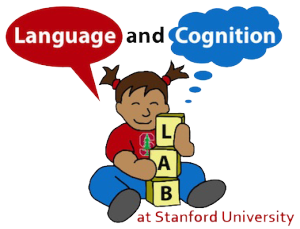
\includegraphics{figs/image-1} 

}

\caption[One column image]{One column image.}\label{fig:image}
\end{figure}
\end{CodeChunk}

\hypertarget{r-plots}{%
\subsection{R Plots}\label{r-plots}}

You can use R chunks directly to plot graphs. And you can use latex
floats in the fig.pos chunk option to have more control over the
location of your plot on the page. For more information on latex
placement specifiers see
\textbf{\href{https://en.wikibooks.org/wiki/LaTeX/Floats,_Figures_and_Captions}{here}}

\begin{CodeChunk}
\begin{figure}[H]

{\centering 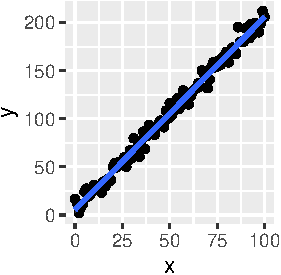
\includegraphics{figs/plot-1} 

}

\caption[R plot]{R plot}\label{fig:plot}
\end{figure}
\end{CodeChunk}

\hypertarget{tables}{%
\subsection{Tables}\label{tables}}

Number tables consecutively; place the table number and title (in 10
point) above the table with one line space above the caption and one
line space below it, as in Table 1. You may float tables to the top or
bottom of a column, set wide tables across both columns.

You can use the xtable function in the xtable package.

\begin{table}[H]
\centering
\begin{tabular}{rrrrr}
  \hline
 & Estimate & Std. Error & t value & Pr($>$$|$t$|$) \\ 
  \hline
(Intercept) & -0.02 & 0.10 & -0.2 & 0.87 \\ 
  x & 1.86 & 0.10 & 17.8 & 0.00 \\ 
   \hline
\end{tabular}
\caption{This table prints across one column.} 
\end{table}

\hypertarget{acknowledgements}{%
\section{Acknowledgements}\label{acknowledgements}}

Place acknowledgments (including funding information) in a section at
the end of the paper.

\hypertarget{references}{%
\section{References}\label{references}}

\setlength{\parindent}{-0.1in} 
\setlength{\leftskip}{0.125in}

\noindent

\hypertarget{refs}{}
\leavevmode\hypertarget{ref-bloom1970language}{}%
Bloom, L. M. (1970). \emph{Language development: Form and function in
emerging grammars} (PhD thesis). Columbia University.

\leavevmode\hypertarget{ref-ChalnickBillman1988a}{}%
Chalnick, A., \& Billman, D. (1988). Unsupervised learning of
correlational structure. In \emph{Proceedings of the tenth annual
conference of the cognitive science society} (pp. 510--516). Hillsdale,
NJ: Lawrence Erlbaum Associates.

\leavevmode\hypertarget{ref-choi1988semantic}{}%
Choi, S. (1988). The semantic development of negation: A
cross-linguistic longitudinal study. \emph{Journal of Child Language},
\emph{15}(3), 517--531.

\leavevmode\hypertarget{ref-darwin1872expression}{}%
Darwin, C. (1998). \emph{The expression of the emotions in man and
animals}. John Murray.

\leavevmode\hypertarget{ref-macwhinney2000childes}{}%
MacWhinney, B. (2000). \emph{The childes project: Tools for analyzing
talk. Transcription format and programs} (Vol. 1). Psychology Press.

\leavevmode\hypertarget{ref-NewellSimon1972a}{}%
Newell, A., \& Simon, H. A. (1972). \emph{Human problem solving}.
Englewood Cliffs, NJ: Prentice-Hall.

\leavevmode\hypertarget{ref-pea1978}{}%
Pea, R. (1978). \emph{The development of negation in early child
language} (PhD thesis). University of Oxford.

\leavevmode\hypertarget{ref-sagae2010morphosyntactic}{}%
Sagae, K., Davis, E., Lavie, A., MacWhinney, B., \& Wintner, S. (2010).
Morphosyntactic annotation of childes transcripts. \emph{Journal of
Child Language}, \emph{37}(3), 705--729.

\bibliographystyle{apacite}


\end{document}
